\begin{table}
    \begin{center}
        \begin{tabular}{ | l | l | l | l | p{5cm} |}
            \hline
            Name & Documents & Features & classes\\ \hline
            20newsgroup & 18000 & 43496 & 6/20 \\ \hline
            reuter50 & 5000 & 29823 & 50 \\ \hline
            \hline
        \end{tabular}
    \end{center}
    \caption{Characteristics of corpora used in the experiments.}
    \label{table:dataset}
\end{table}
%%%%%%%%%%%%%%%%%%%%%%%%%%%%%%%%%%%%%%%%%%%%%%%%%%%%%%%%%%%%%%%%%%%%%%%%%%%
\subsection{Results} 
%%%%%%%%%%%%%%%%%%%%%%%%%%%%%%%%%%%%%%%%%%%%%%%%%%%%%%%%%%%%%%%%%%%%%%%%%%%
In order to evaluate our proposal, we ran experiments over two standard corpora, namely: 20Newsgroup\footnote{http://qwone.com/\~jason/20Newsgroups} and Reuter50\footnote{https://archive.ics.uci.edu/ml/datasets/Reuter\_50\_50}.
%The first one consists of 13000 messages taken from 20 newsgroups, whereas the second one contains 5000 documents authored by 50 different authors. 
Table~\ref{table:dataset} summarises the characteristics of the two corpora. Each corpus is divided in a training and test set with a ratio 80-20 percent. Models are evaluated according to their perplexity on the test set and we follow here the  approach of \cite{asuncion_smoothing_2009} based on the following fold-in procedure: the topic-word distribution is learned on the training set and considered fixed, whereas the document-topic distribution is learned for each document of the test set, by using the first half of the document only. The perplexity is then computed on each test document, then averaged over all test documents, using:
\begin{eqnarray*}
    \textrm{perplexity} & = & \exp-\frac{\sum_{dw}n_{dw}\log\tilde{p}(w|d)}{\sum_{dw}n_{dw}}
\end{eqnarray*}
where the index $d$ in the sums ranges over the test documents only, and the numerator is replaced by its lower bound obtained from~(\ref{eqn:perplex-bound}).

Based on this perplexity measure, we have compared several variants of the LDA model discussed above: $(i)$ with a symmetric prior, fixed or estimated with the EM type 2 procedure, for $\alpha$ and/or $\beta$; $(ii)$ with a fixed asymmetric prior, for $\alpha$ and/or $\beta$; $(iii)$ with a full conjugate prior, for $\alpha$ and/or $\beta$.

The best combination is obtained with a fixed asymmetric prior on $\alpha$ and full conjugacy on $\beta$. In the remainder, we refer to this model as {\em conjugate LDA}. Both full conjugacy and the asymmetric prior on $\alpha$ yield better results than the symmetric one, in accordance with the results obtained in~\cite{wallach_rethinking_2009} which illustrate the importance of an asymmetric prior on the document-topic distribution. Furthermore, full conjugacy yields better results than an asymmetric prior.

\begin{figure}[ht]
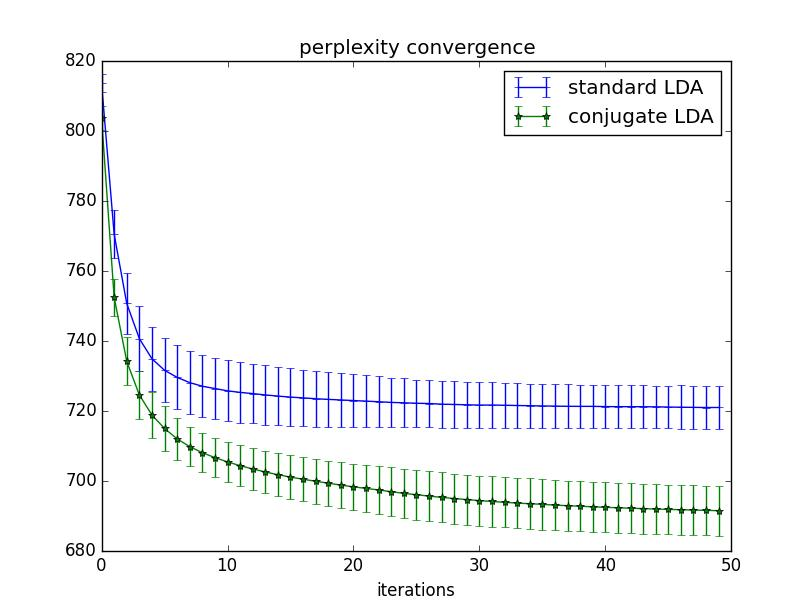
\includegraphics[scale=0.4]{results/pp_conv}
\caption{\label{fig:pp-exple}Evolution of perplexity on the test sets according to the number of iterations of the variational Bayes methods for both conjugate and standard LDA, on 20Newsgroup.}
\end{figure}
Figure~\ref{fig:pp-exple} illustrates the behaviour of the conjugate LDA model wrt to the standard LDA model (with symmetric priors estimated via the EM type 2 procedure). The perplexity is averaged over 10 runs to assess the influence of the random initialisation of the parameters. The number of topics is set to 6 and the number of documents to 1000. Observe that the perplexity of the full conjugacy model is lower than that of the standard model, and decreases with the number of iterations, as expected. Full conjugacy on the word-topic side leads to a higher decrease in perplexity.

\begin{figure}[ht]
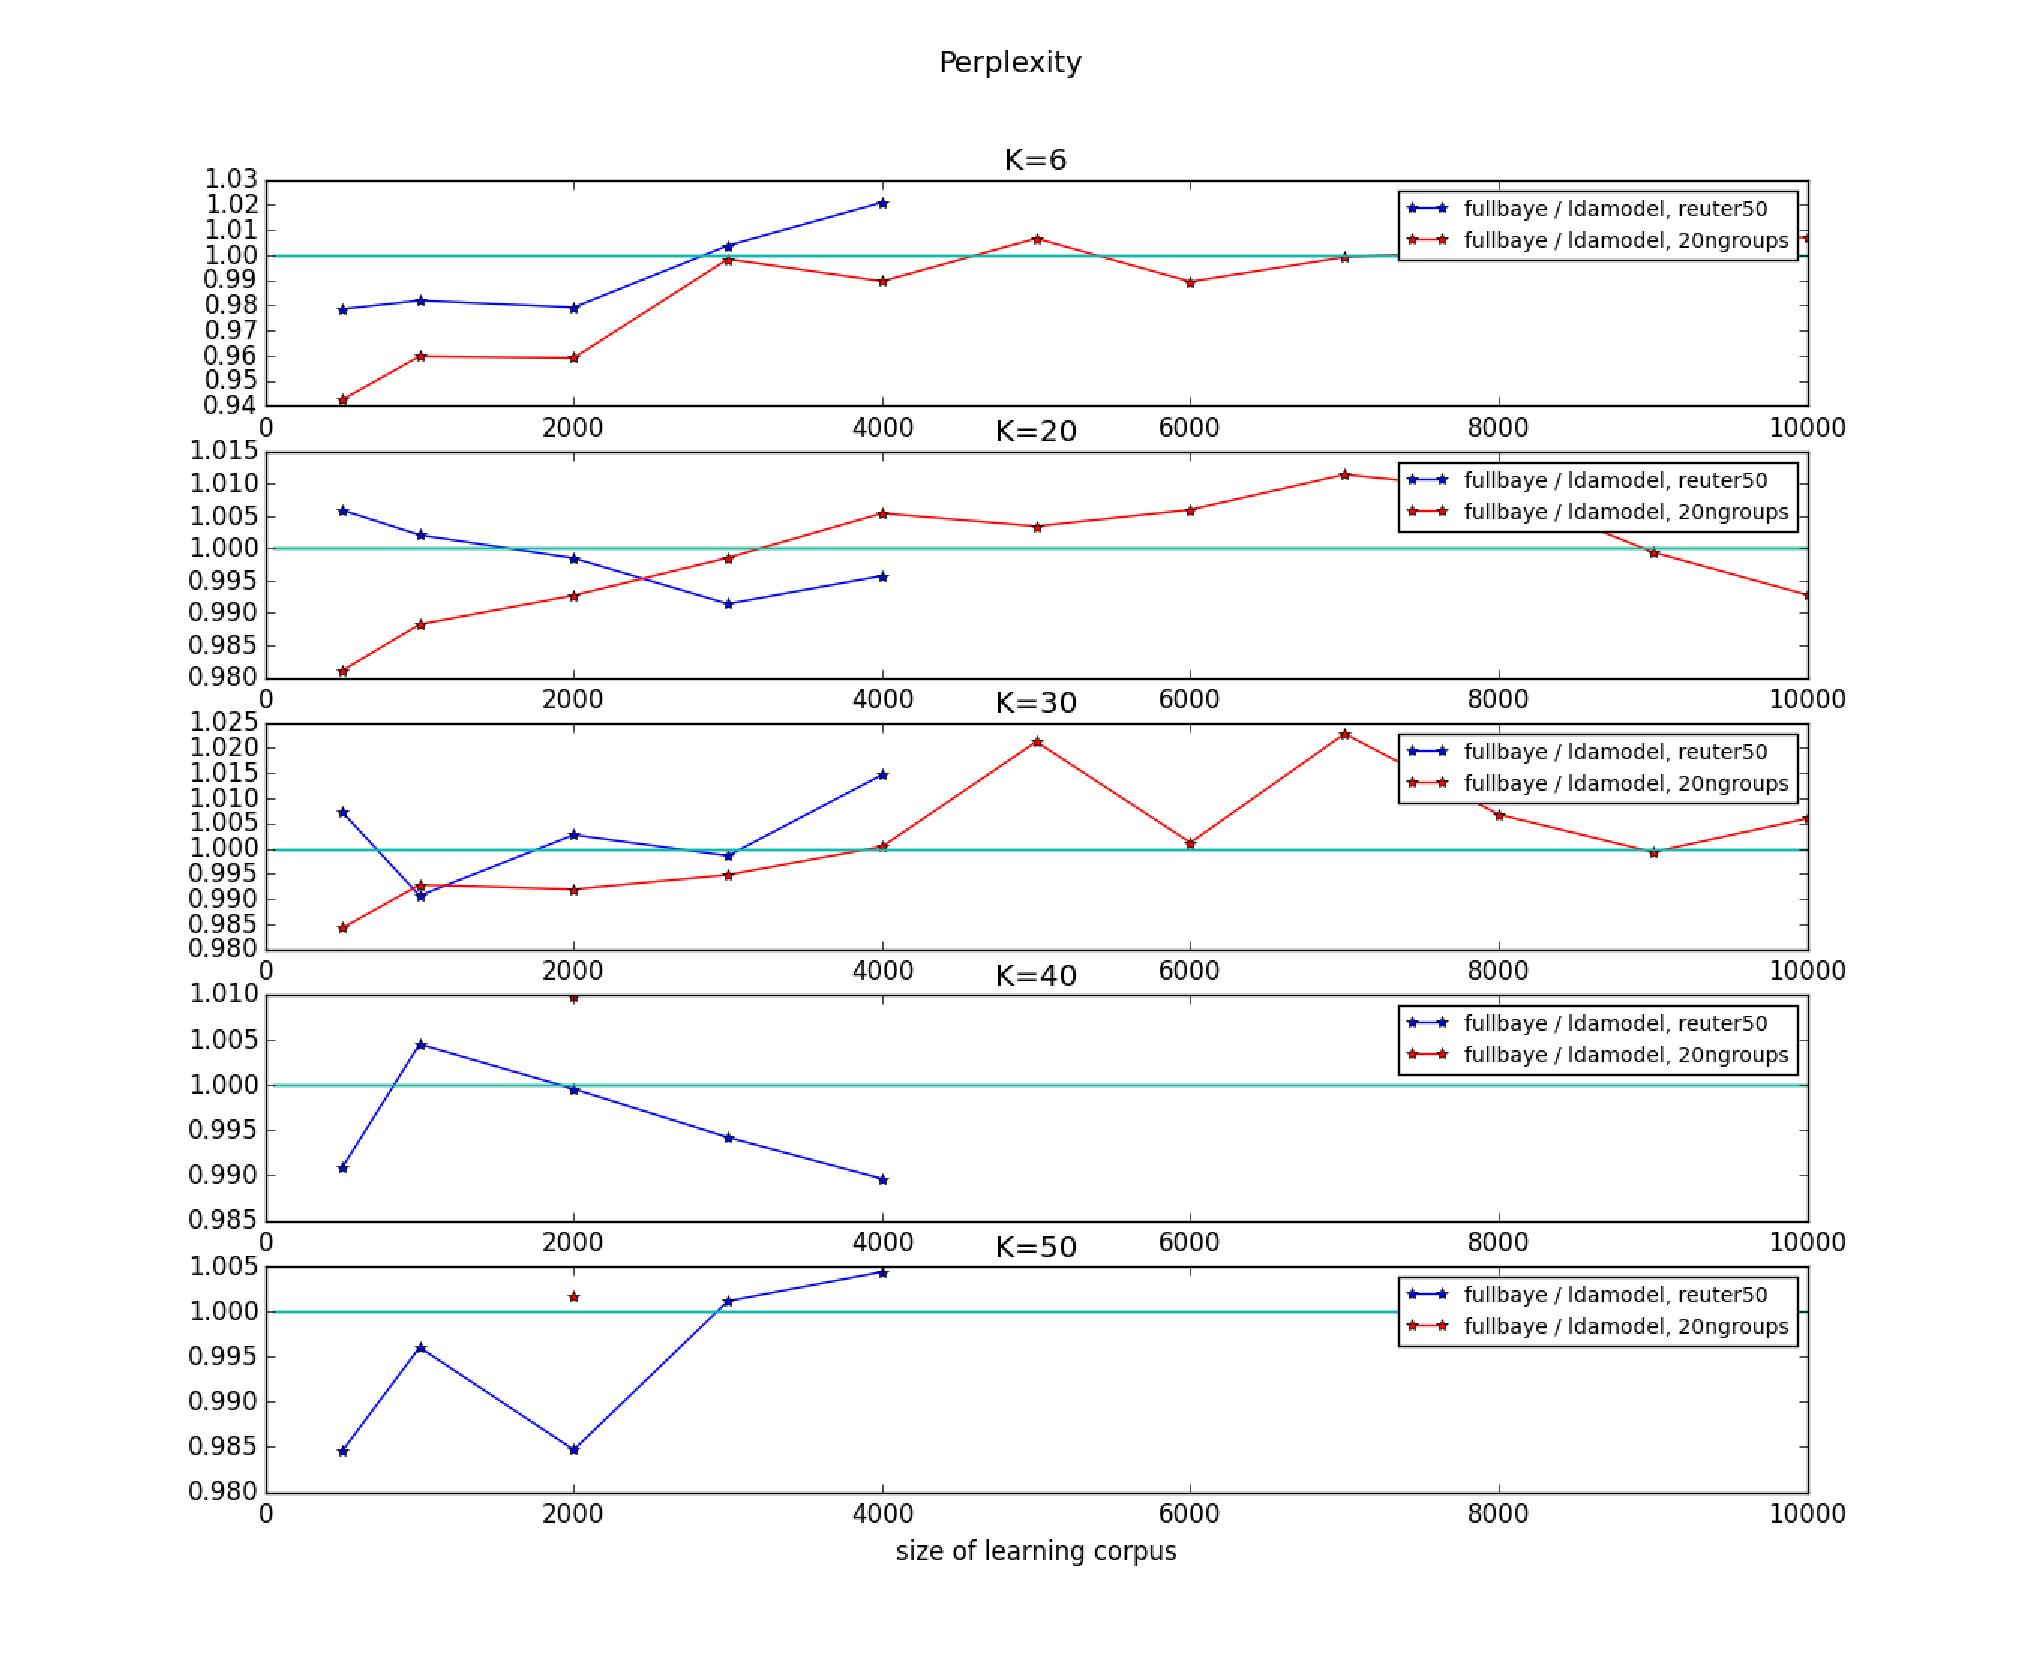
\includegraphics[width=9cm, height=14cm]{results/pp_D}
\caption{(b) \label{fig:pp-size}Perplexity ratio for the conjugate LDA model and the standard LDA model according to the size of the collection ($K=6,20$ for 20 Newsgroup and $K=6,50$ for Reuter50).}
\end{figure}
Figure~\ref{fig:pp-size} shows how the conjugate LDA model behaves, compared to the standard LDA model, with respect to the size of the collection. Here again, the number of topics $K$ is first set to $6$ and the curves correspond to the ratio of perplexity of the conjugate LDA model w.r.t. to the standard LDA model. Observe that the perplexity ratio is below $1$ for smaller collections (ca. below 3000 documents). This indicates that the conjugate LDA model compares favourably to the standard model for small collections, which can be explained by the additional information brought by the prior on such collections (the influence of the prior then decreases with the size of the collection).
%Figure~\ref{fig:pp_D} also displays the ratio of perplexity for the two collections with the number of topics set to the actual number of classes in the collections: $K=20$ for 20 Newsgroup, as the data originates from $20$ different news groups, and $K=50$ for Reuter50 as the texts are authored by $50$ different persons. As one can note, we observe the same tendency as the one mentioned above, even though the difference between the two models is less marked.

%\textcolor{red}{To be kept and completed if we have a nice illustration!\\ Figure~\ref{fig:3} illustrates the qualitative impact of the Boojum prior on the word-topic distribution.}

\begin{figure}[ht]
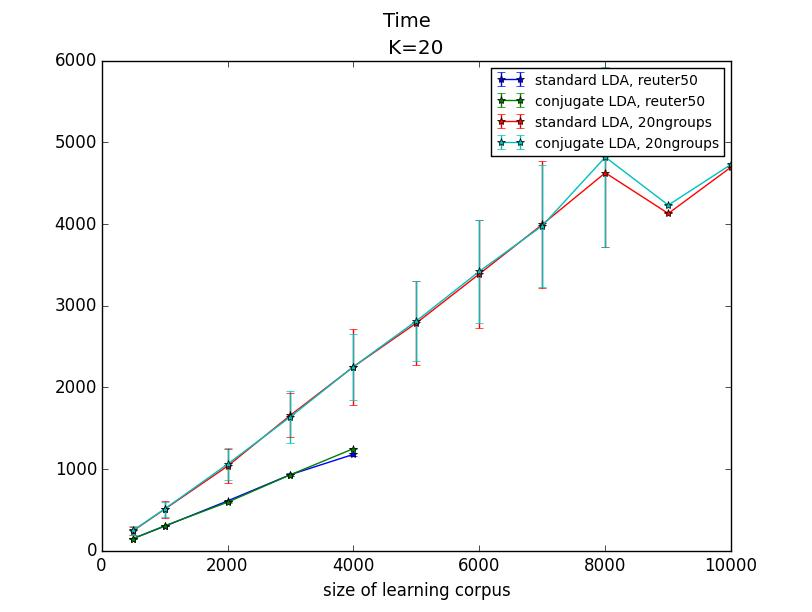
\includegraphics[scale=0.4]{results/time}
\caption{\label{fig:time}Time of inference for 50 iterations of variational bayes.}
\end{figure}
Finally, Figure~\ref{fig:time} compares the execution time of the inference procedures for the two models for $K=20$. Similar plots are obtained for different values of $K$. There is no significant difference between the inference time in the conjugate and the standard models.
